\documentclass[fontset=windows]{article}
\usepackage[]{ctex}
\usepackage[a4paper, total={6in, 8in}]{geometry}

\title{基数树 项目报告}
\author{楼天驰 522031910290}
\date{2024年 4月 25日}

\usepackage{natbib}
\usepackage{graphicx}
\usepackage{enumitem}
\usepackage{subfigure}
\bibliographystyle{plain}

\begin{document}

\maketitle
    
\section{背景介绍}
RadixTree是一种多叉树,通过共享一段文本或字节码的前缀来节省储存空间。在本Project中,将存储int32\_t(32位整型)的数据,以其二进制码的共同前缀来节省空间,使用一棵4叉树。

RadixTree可以通过节点压缩进行优化。具体而言,如果有冗余的节点(如只有一个子节点),则可以将其合并,同时记录其具体数值。在这个操作后可以降低树的高度,减少节点数量,从而使查询的延迟减小,但是可能使插入与删除操作的时间增加。由于插入与删除操作中也隐含了查询操作,因此总体而言,插入和删除操作的延迟也是减小的。

\section{系统实现}
在本节中,简单描述了Radix Tree与Compressed Radix Tree的实现细节,列举了实现过程中的一些难点。
\subsection{Radix Tree}
基础的Radix Tree的实现不算困难。

一棵Radix Tree中的变量主要有:根节点指针,树的高度、大小。

主要的方法有:构造与析构函数,插入(insert)函数,查找(find)函数,删除(remove)函数,查询高度(height)函数,查询大小(size)函数。
\subsubsection{节点}
在基础的Radix Tree的实现中,一个Radix Node中包括的信息有:父亲节点的指针、四个孩子节点的指针(如果没有即为nullptr)、孩子节点数。

在创建一个结点时传入并保持父亲节点的指针,同时将孩子节点指针均设为nullptr.

\subsubsection{基本操作}
查询:类似于其他查找树,每次以当前剩余数值二进制表示中的前两位作为index,访问此index下的子节点,直到访问的结点为空。如果要访问的节点不存在,则代表着当前查找的这个key在Radix Tree中不存在。

插入:预备的操作与查询类似,区别是如果有不存在的节点,则创建一个新的节点(注意修改高度和大小);如果此节点以存在,则跳到这个节点上,继续后续操作。

删除:先进行一次查询,找到要删除的点(不存在就直接return)。在找到此节点后,自底向上开始修改,如果此节点没有孩子,则删除此结点,并且修改父亲节点孩子数量。

高度与大小:在插入、删除的同时维护。由于Radix Tree的实现比较基础,高度的取值只有两个,因此只考虑根有孩子与根没有孩子的两种情况即可。

\subsection{Compressed Radix Tree}

\subsubsection{节点}
与基础的Radix Tree基本一致,新增了高度记录,当前结点值记录,当前结点值长度记录。新增了一个update方法,用于从本身的孩子节点更新当前节点的高度。

\subsubsection{基本操作}
查询:与之前基本一致,在每次尝试向孩子节点转移时判断传入的value中的这一段数值与孩子节点储存的value是否一致,如果不一致则说明当前树中不存在要查询的值。在这部分中,要注意截取具体数值时,用左移操作时的数字 1 要用 1ull 代替,不然会出现溢出的问题。

插入:在基础的Radix Tree的基础上修改了新增结点的操作,新增结点不再继续分裂,而是直接保存在新构建出的节点中。新增了分裂的操作,这部分在后续会具体展开。

删除:在基础的Radix Tree的基础上增加了当一个节点只有一个孩子的将孩子节点与此节点合并的操作。同时增加了以较低时间复杂度更新高度的操作。

\subsection{实现过程中的难点}
在Compressed Radix Tree的实现过程中,我在插入操作中的分裂操作中的调试花费了大量的时间。首先,在分裂时不能改变原有结点的孩子的结构,因此有一个小的技巧,将当前结点下放,新增一个父亲节点和一个兄弟结点,从而减少拷贝的次数,同时不再需要交换操作。其次,在分裂后每个节点的值的长度可能是不相同的,这一步需要想清楚再写,或者多用几个中间变量使逻辑更加清晰,从而减少错误的发生。最后,要注意循环引用的问题,在修改指向父亲、孩子的指针时要考虑清楚。

在Compressed Radix Tree的实现中,统计树的高度是一个重难点,我考虑了三种统计的方式:
\begin{enumerate}
  \item 直接在要求返回高度时,遍历整棵树来找出最深的结点,从而找出树高。但是如果此函数调用次数多的话会导致性能严重下降。
  \item 记录每个高度的节点数量,从而可以在常数的时间复杂度内返回高度,但是如果一个父节点的高度改变(如结点合并导致的),会导致整棵子树都要修改。
  \item 自底向上,每次将有修改的节点的高度向上更新,父节点的高度即为子节点高度最大值再加一。每次修改最多影响一条链,时间复杂度为常数。查询时返回根的高度即可。
\end{enumerate}
最终经过对比,选择了第三种方式。

\section{测试}
此部分主要展现本项目的测试,主要分为正确性测试与YCSB性能测试两个子部分。

\subsection{正确性测试}
使用已经提供的测试脚本grade.sh,运行make grade进行正确性测试如图~\ref{fig:Grade}。Radix Tree 与 Compressed Radix Tree均通过了正确性测试。

\begin{figure}[h!]
  \centering
  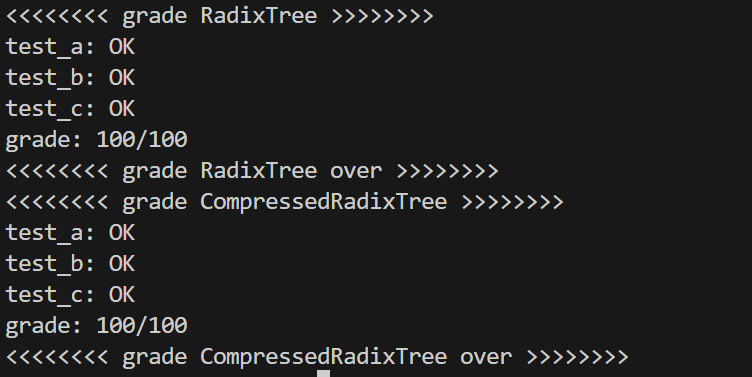
\includegraphics[width=0.5\textwidth]{grade}
  \caption{Correctness Test Result}
  \label{fig:Grade}

\end{figure}

\subsection{YCSB测试}

\subsubsection{测试配置}

工作负载:按插入、查找、删除所占的比例不同分为以下三类:
\begin{enumerate}
  \item 插入50\%,查找50\%
  \item 查找100\%
  \item 插入25\%,查找50\%,删除25\%
\end{enumerate}

测试对象:Radix Tree,Compressed Radix Tree,Red-Black Tree\footnote{来源为oi-wiki https://oi-wiki.org/ds/llrbt/}。

测试环境:OpenEuler CPU数:2 内存:8G 

\subsubsection{测试结果}

\begin{figure} [h!]
\centering
\subfigure[Workload1 Result] {
  \centering
  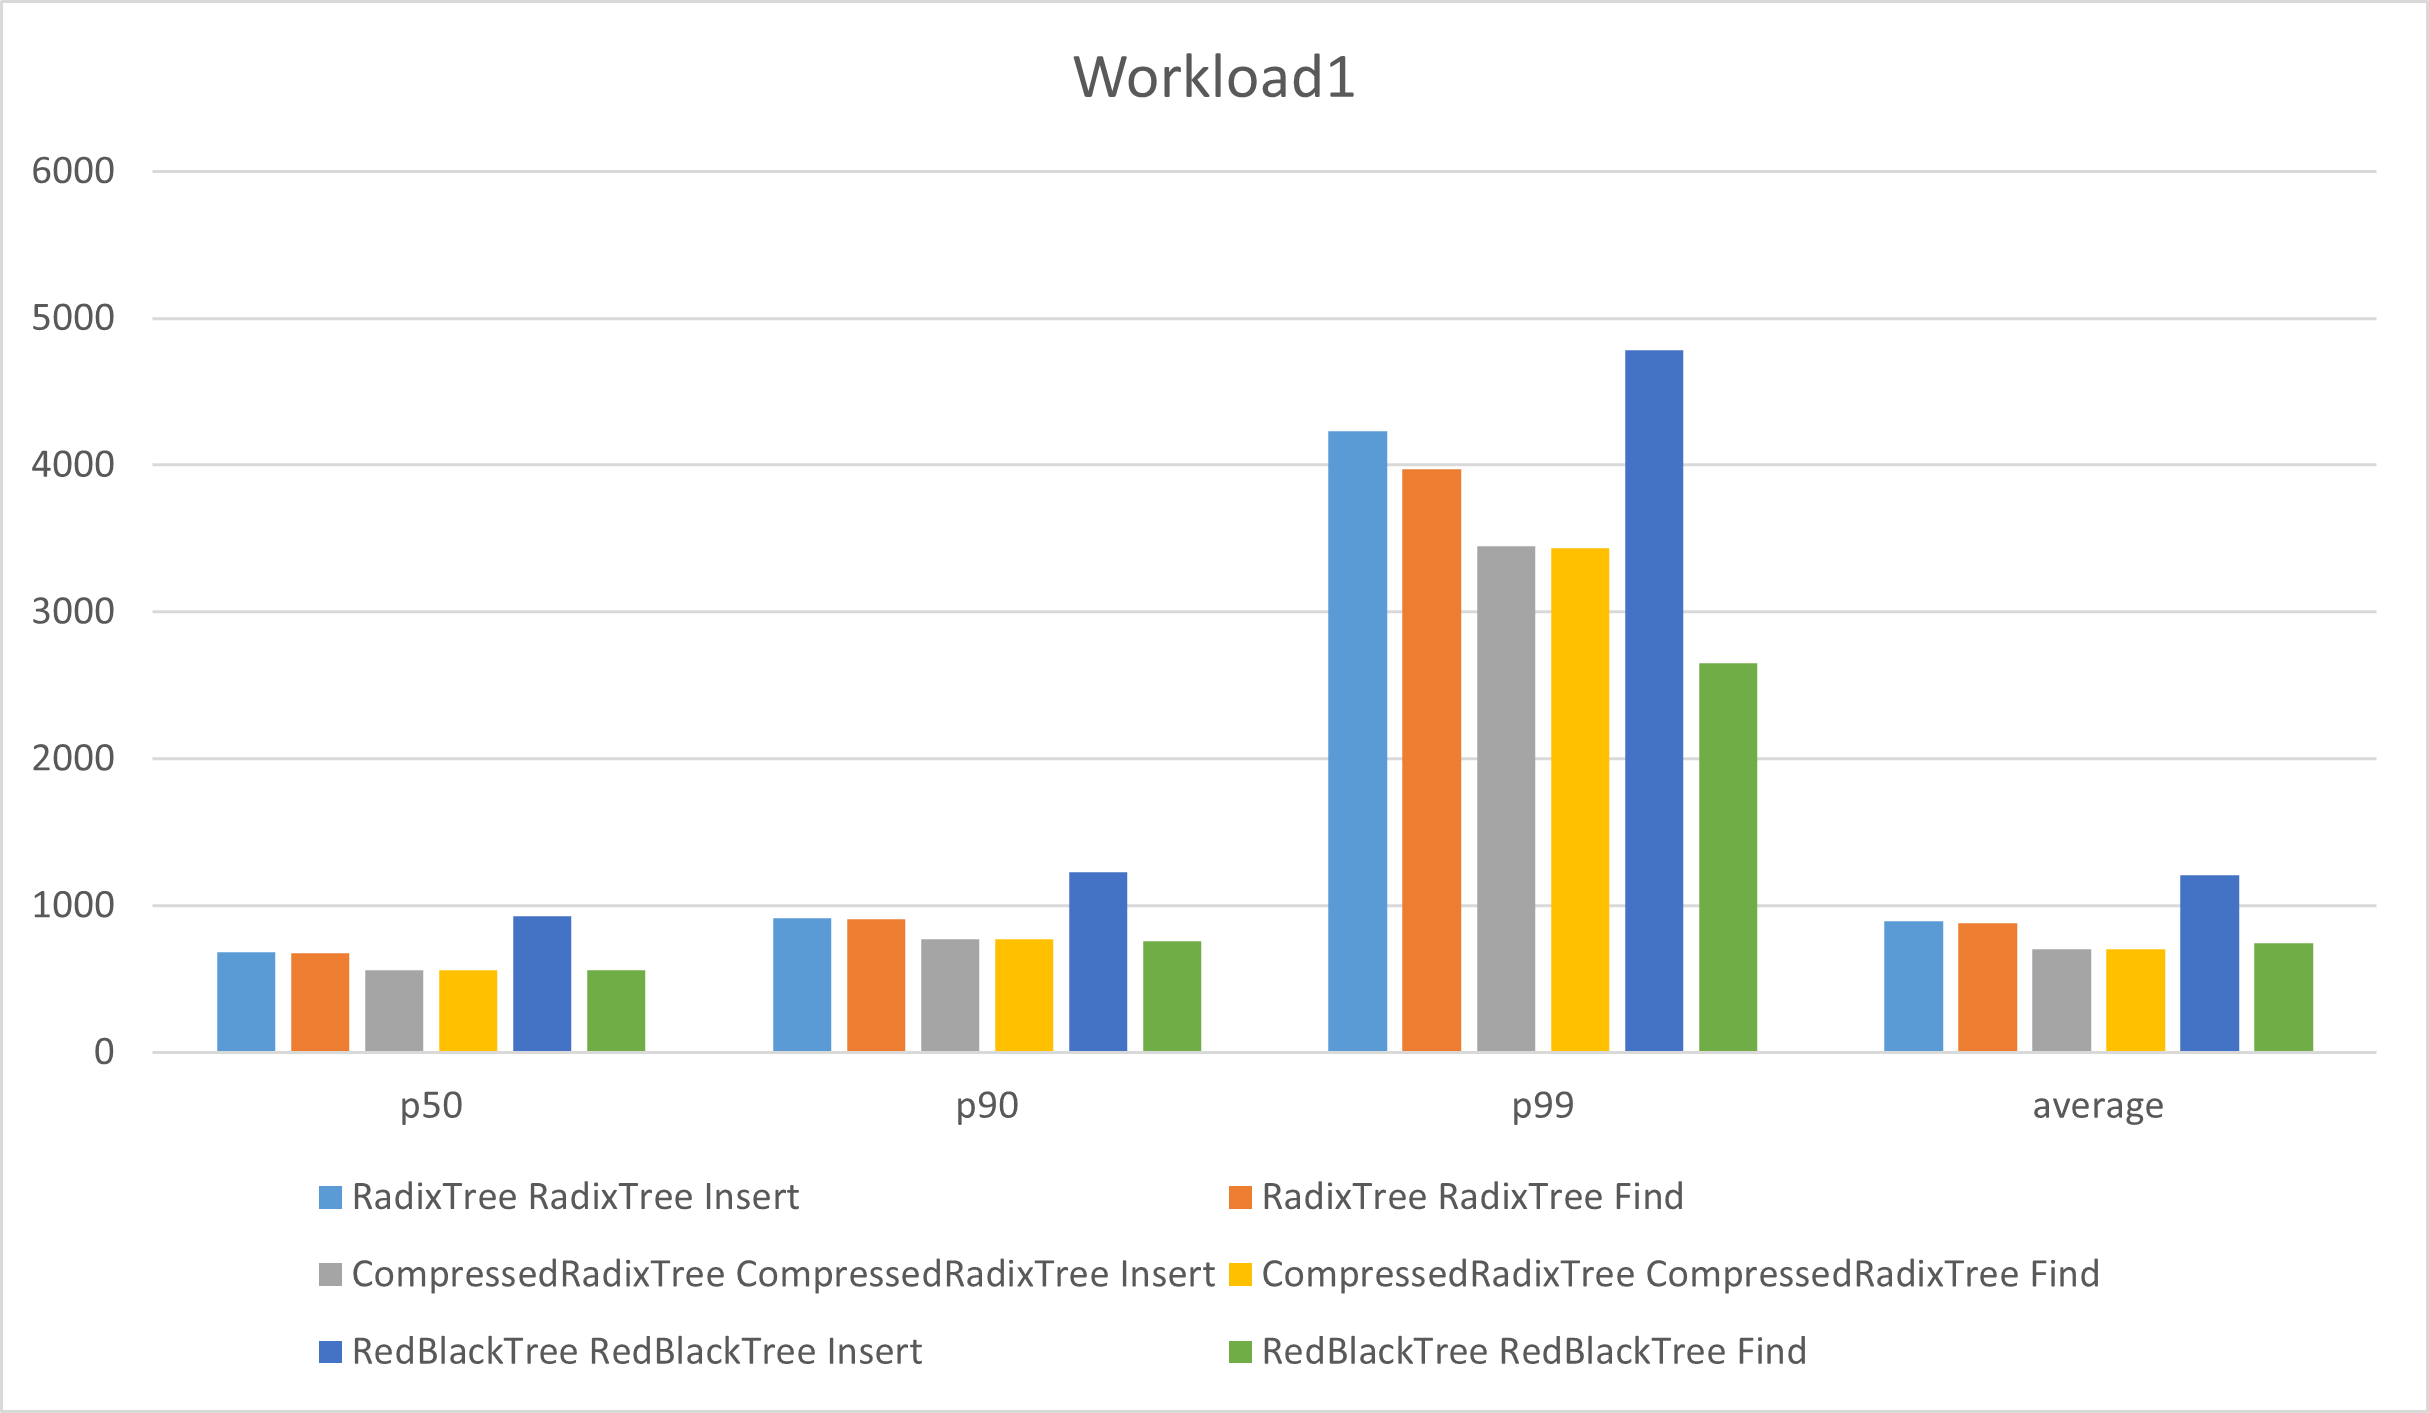
\includegraphics[width=0.29\textwidth]{workload1}
  \label{fig:workload1}
}
\subfigure[Workload2 Result] {
  \centering
  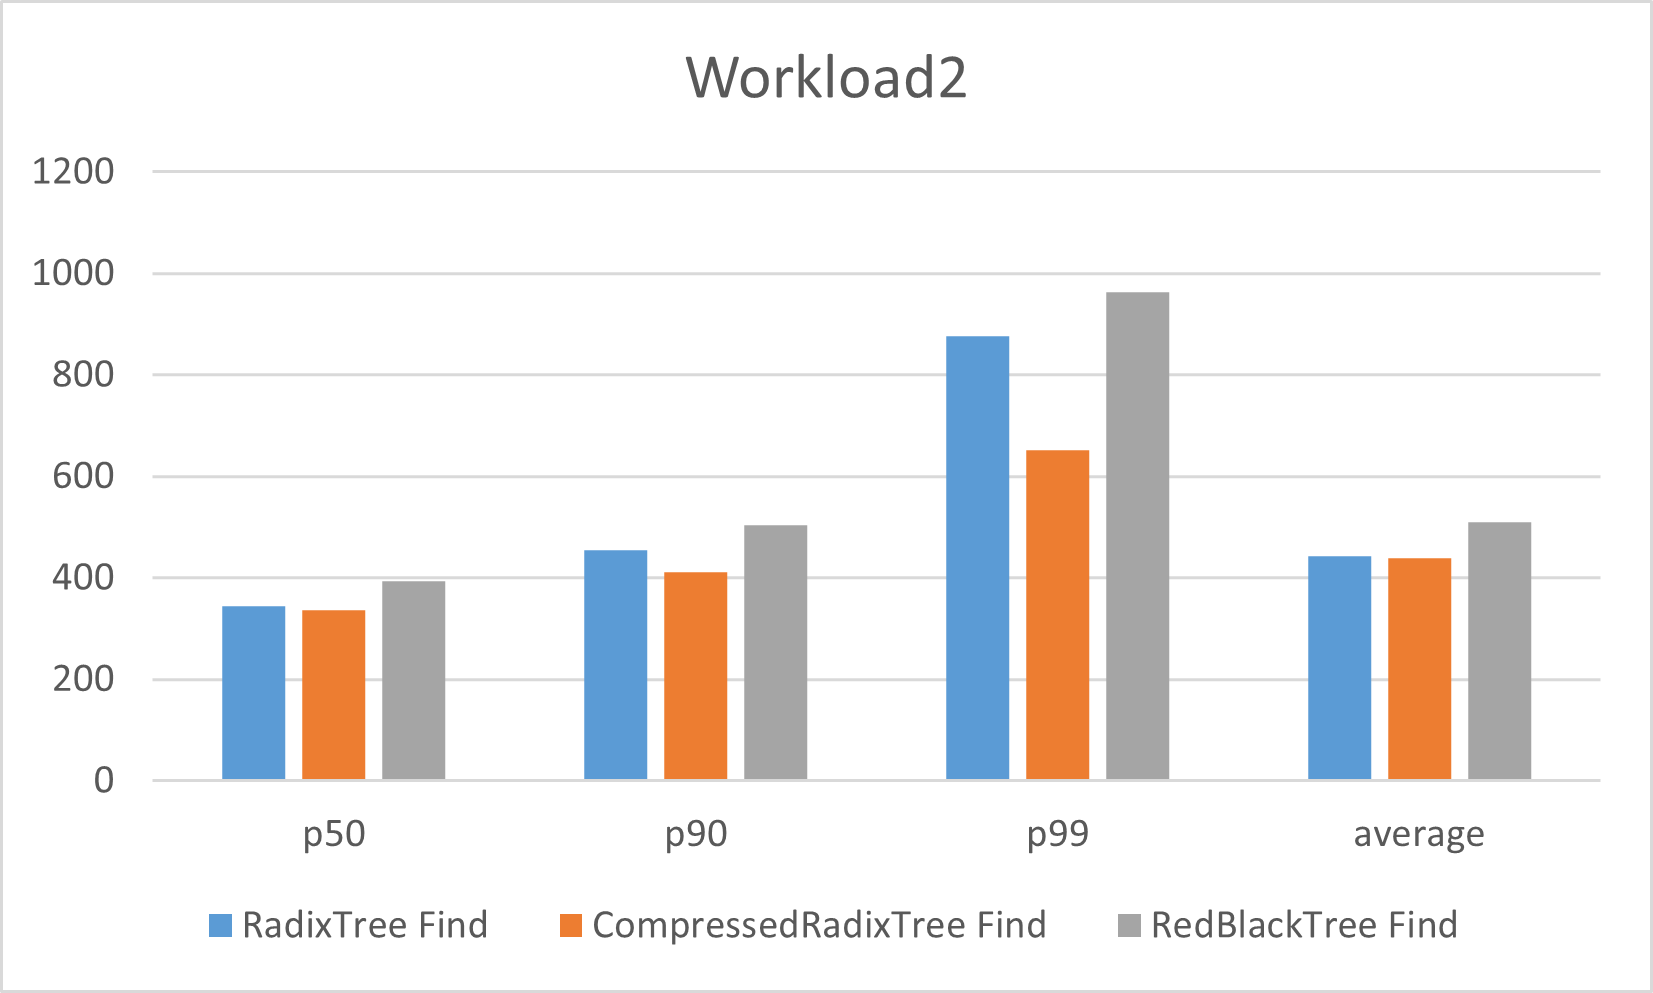
\includegraphics[width=0.28\textwidth]{workload2}
  \label{fig:workload2}
}
\subfigure[Workload3 Result] {
  \centering
  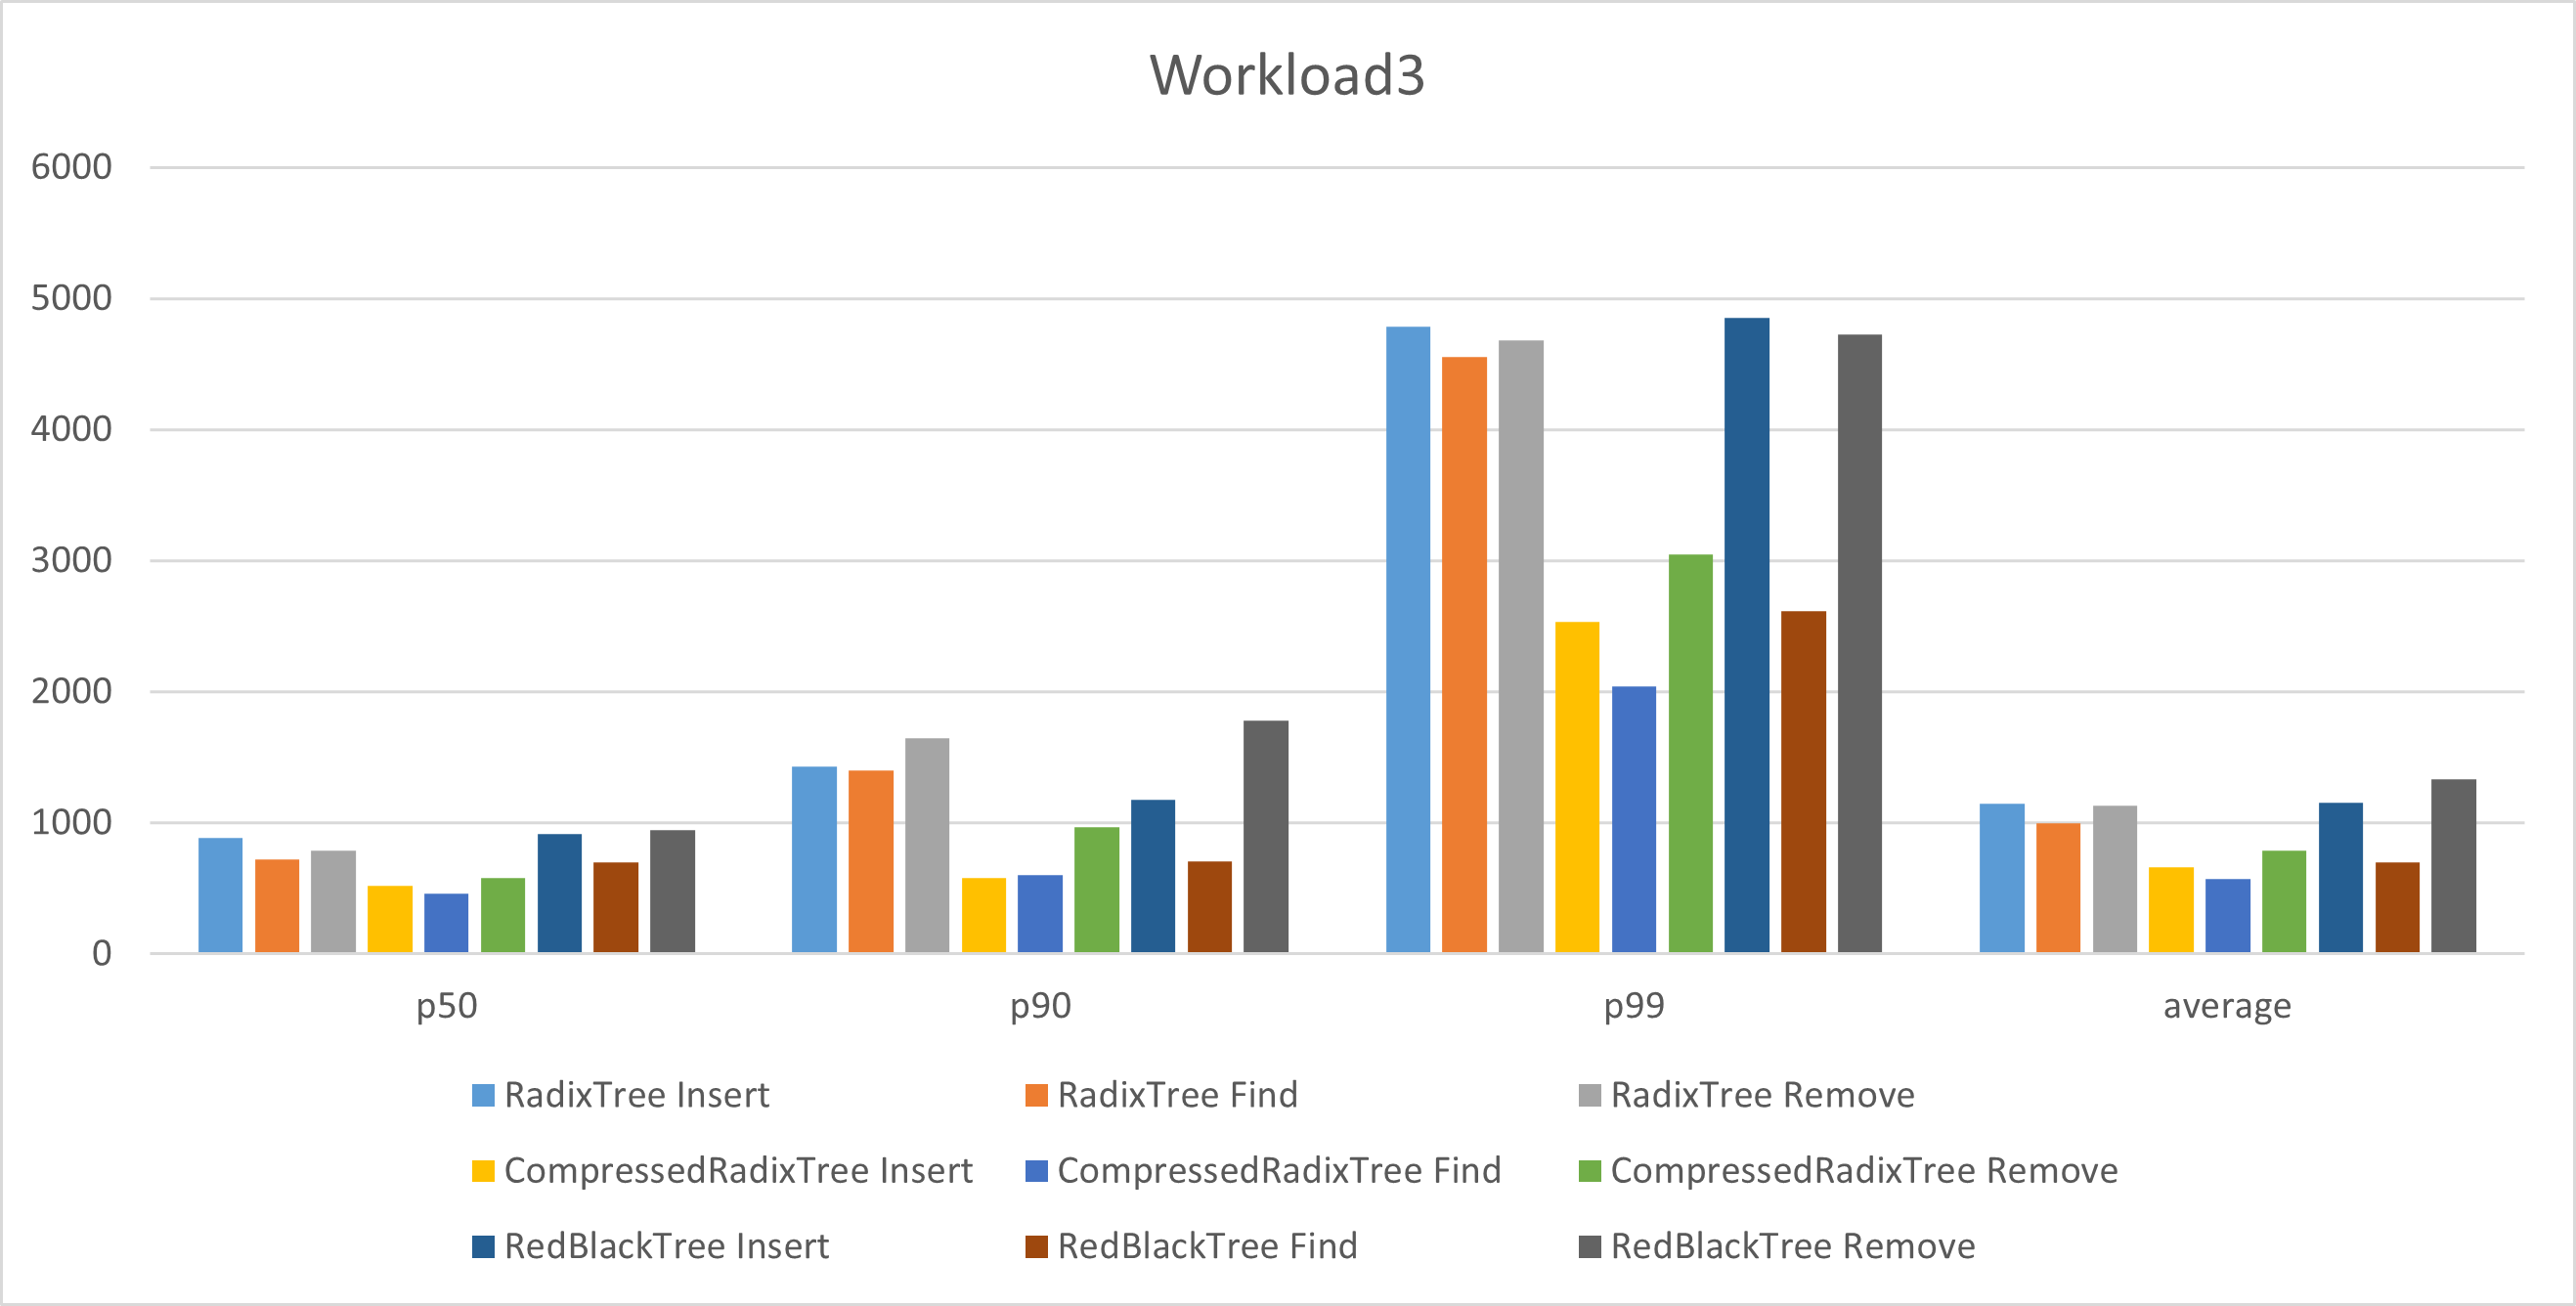
\includegraphics[width=0.33\textwidth]{workload3}
  \label{fig:workload3}
}
\caption{YCSB Test Result}
\label{fig:ycsbResult}
\end{figure}
对workload1、2、3的测试结果见图~\ref{fig:ycsbResult},实验结果符合我们的预期。

\subsubsection{结果分析}
从中,我们可以看到Compressed Radix Tree在三种工作负载中的三种不同操作,P50、P90、P99与平均时延的指标都是最优的,尤其是在高百分位数的延迟情况下,这可能意味着它在高负载或者数据量大的场景下具备更好的稳定性。而未压缩的Radix Tree对红黑树没有体现出很大的优势,但是在查找操作方面表现良好。而红黑树在这种场景下的表现并不突出,可能是由于维持平衡的性能开销的影响。

\section{结论}
这个 Project 锻炼了我的编码能力,对Radix Tree及其优化版本Compressed Radix Tree的实现有了深入的了解。同时,通过YCSB的测试编写,不仅锻炼了我的测试能力,了解了怎么写一个更加通用从而更加方便的测试,也对Radix Tree的具体使用场景与操作的时延有了更深的理解。总的来说,Radix Tree有高效的空间利用率和快速的搜索性能,在储存诸如词典这样有大量信息的场景下表现优秀,特别是那些需要高效率查找、插入和删除的字符串集合的应用场合。


\end{document}
